\begin{figure}[H]
\centering
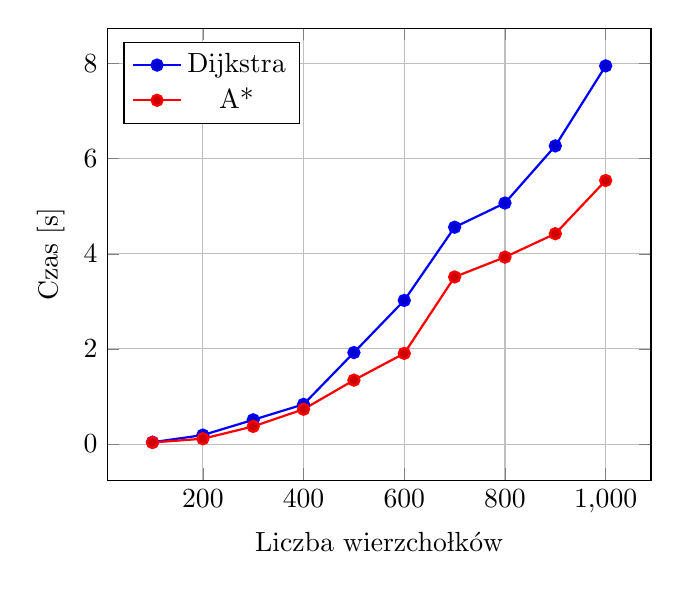
\begin{tikzpicture}
\begin{axis}[
xlabel = {Liczba wierzchołków},
ylabel = {Czas [s]},
legend pos = north west,
grid = both,
width=0.7\linewidth,
]
\addplot + [mark = *, thick] coordinates
    {
(100, 0.038941144943237305)(200, 0.18861889839172363)(300, 0.5098412036895752)(400, 0.8351962566375732)(500, 1.9239015579223633)(600, 3.0202627182006836)(700, 4.5584397315979)(800, 5.066880702972412)(900, 6.268101215362549)(1000, 7.950292348861694)};
\addlegendentry
{Dijkstra}
\addplot + [mark = *, thick] coordinates
    {
(100, 0.034009695053100586)(200, 0.11242508888244629)(300, 0.37114644050598145)(400, 0.731886625289917)(500, 1.344003438949585)(600, 1.9063656330108643)(700, 3.512908697128296)(800, 3.9297196865081787)(900, 4.422373294830322)(1000, 5.540976047515869)};
\addlegendentry
{A*}
\end{axis}
\end{tikzpicture}
\caption
{Porównanie czasów działania algorytmów Dijkstry i A* (duże instancje)}
\label{fig:shortest_path_chart}
\end{figure}
